\section{Polarization primer} \label{sec:pol-primer}
\subsection{Constructing $E/B$ fields without harmonic space}
%\comment{Need a better title for the section that gives the heuristic argument}
%\textit{Alternative for bringing the heuristic argument earlier.}

 CMB polarization is measured in terms of Stokes parameters, time averages of the linear polarization of the electric field along cartesian axes perpendicular to the line of sight.\footnote{Throughout we use the conventions of HEALPix \cite{healpix_primer}, measuring the polarization angle East of South.} Thus Stokes $Q$ and $U$ depend on the choice of the local coordinate system, and a rotation by an angle $\psi$ around the line of sight transforms them as
%
\beq \label{eq:qu-rot}
\fqu' = \begin{bmatrix} \cos{2 \phi} &  \sin{2 \phi} \\ -\sin{2\phi} & \cos{2 \phi} \end{bmatrix} \fqu \,.
\eeq
Equivalently the object $_{\pm 2}\bar{X}(\hat{n}) = Q(\hat{n}) \pm i U (\hat{n})$ transforms as ${}_{\pm 2}f' = e^{\mp 2i\phi} {}_{s}f$ and hence forms a spin-2 field \cite{Zaldarriaga1997}.

The standard construction of $E$ and $B$ fields arise from the desire to have a coordinate independent description of the polarization. This follows from operations that raise (or lower) the spin of the $X$ field to construct scalar fields.  But from the transform properties of the Stokes parameters, we can already construct a heuristic argument for what these operations must look like in real space.

We consider the contribution to a scalar field at $\hat n_e$ from the polarization field at $\hat n_q$. \fig{fig:euler_angles} shows that the transformation of the local coordinate system between the two positions can be described by a rotation around the local $\hat n_q$ by angle $\alpha$, parallel transport by angle $\beta$, and a rotation around $\hat n_q$ by $-\gamma$.  This corresponds to a rotation by Euler angles $(\alpha,\beta,-\gamma)$ in the $z-y_1-z_2$ convention.\footnote{The Euler angles in the more standard $z-y-z$ convention are related to those in the $z-y_1-z_2$ convection by the following rule: $(\alpha,\beta,\gamma)_{z-y-z} =(\gamma,\beta,\alpha)_{z-y_1-z_2}$ \cite{varshalovich}.}
%
\begin{figure}%[!hbt]
\centering
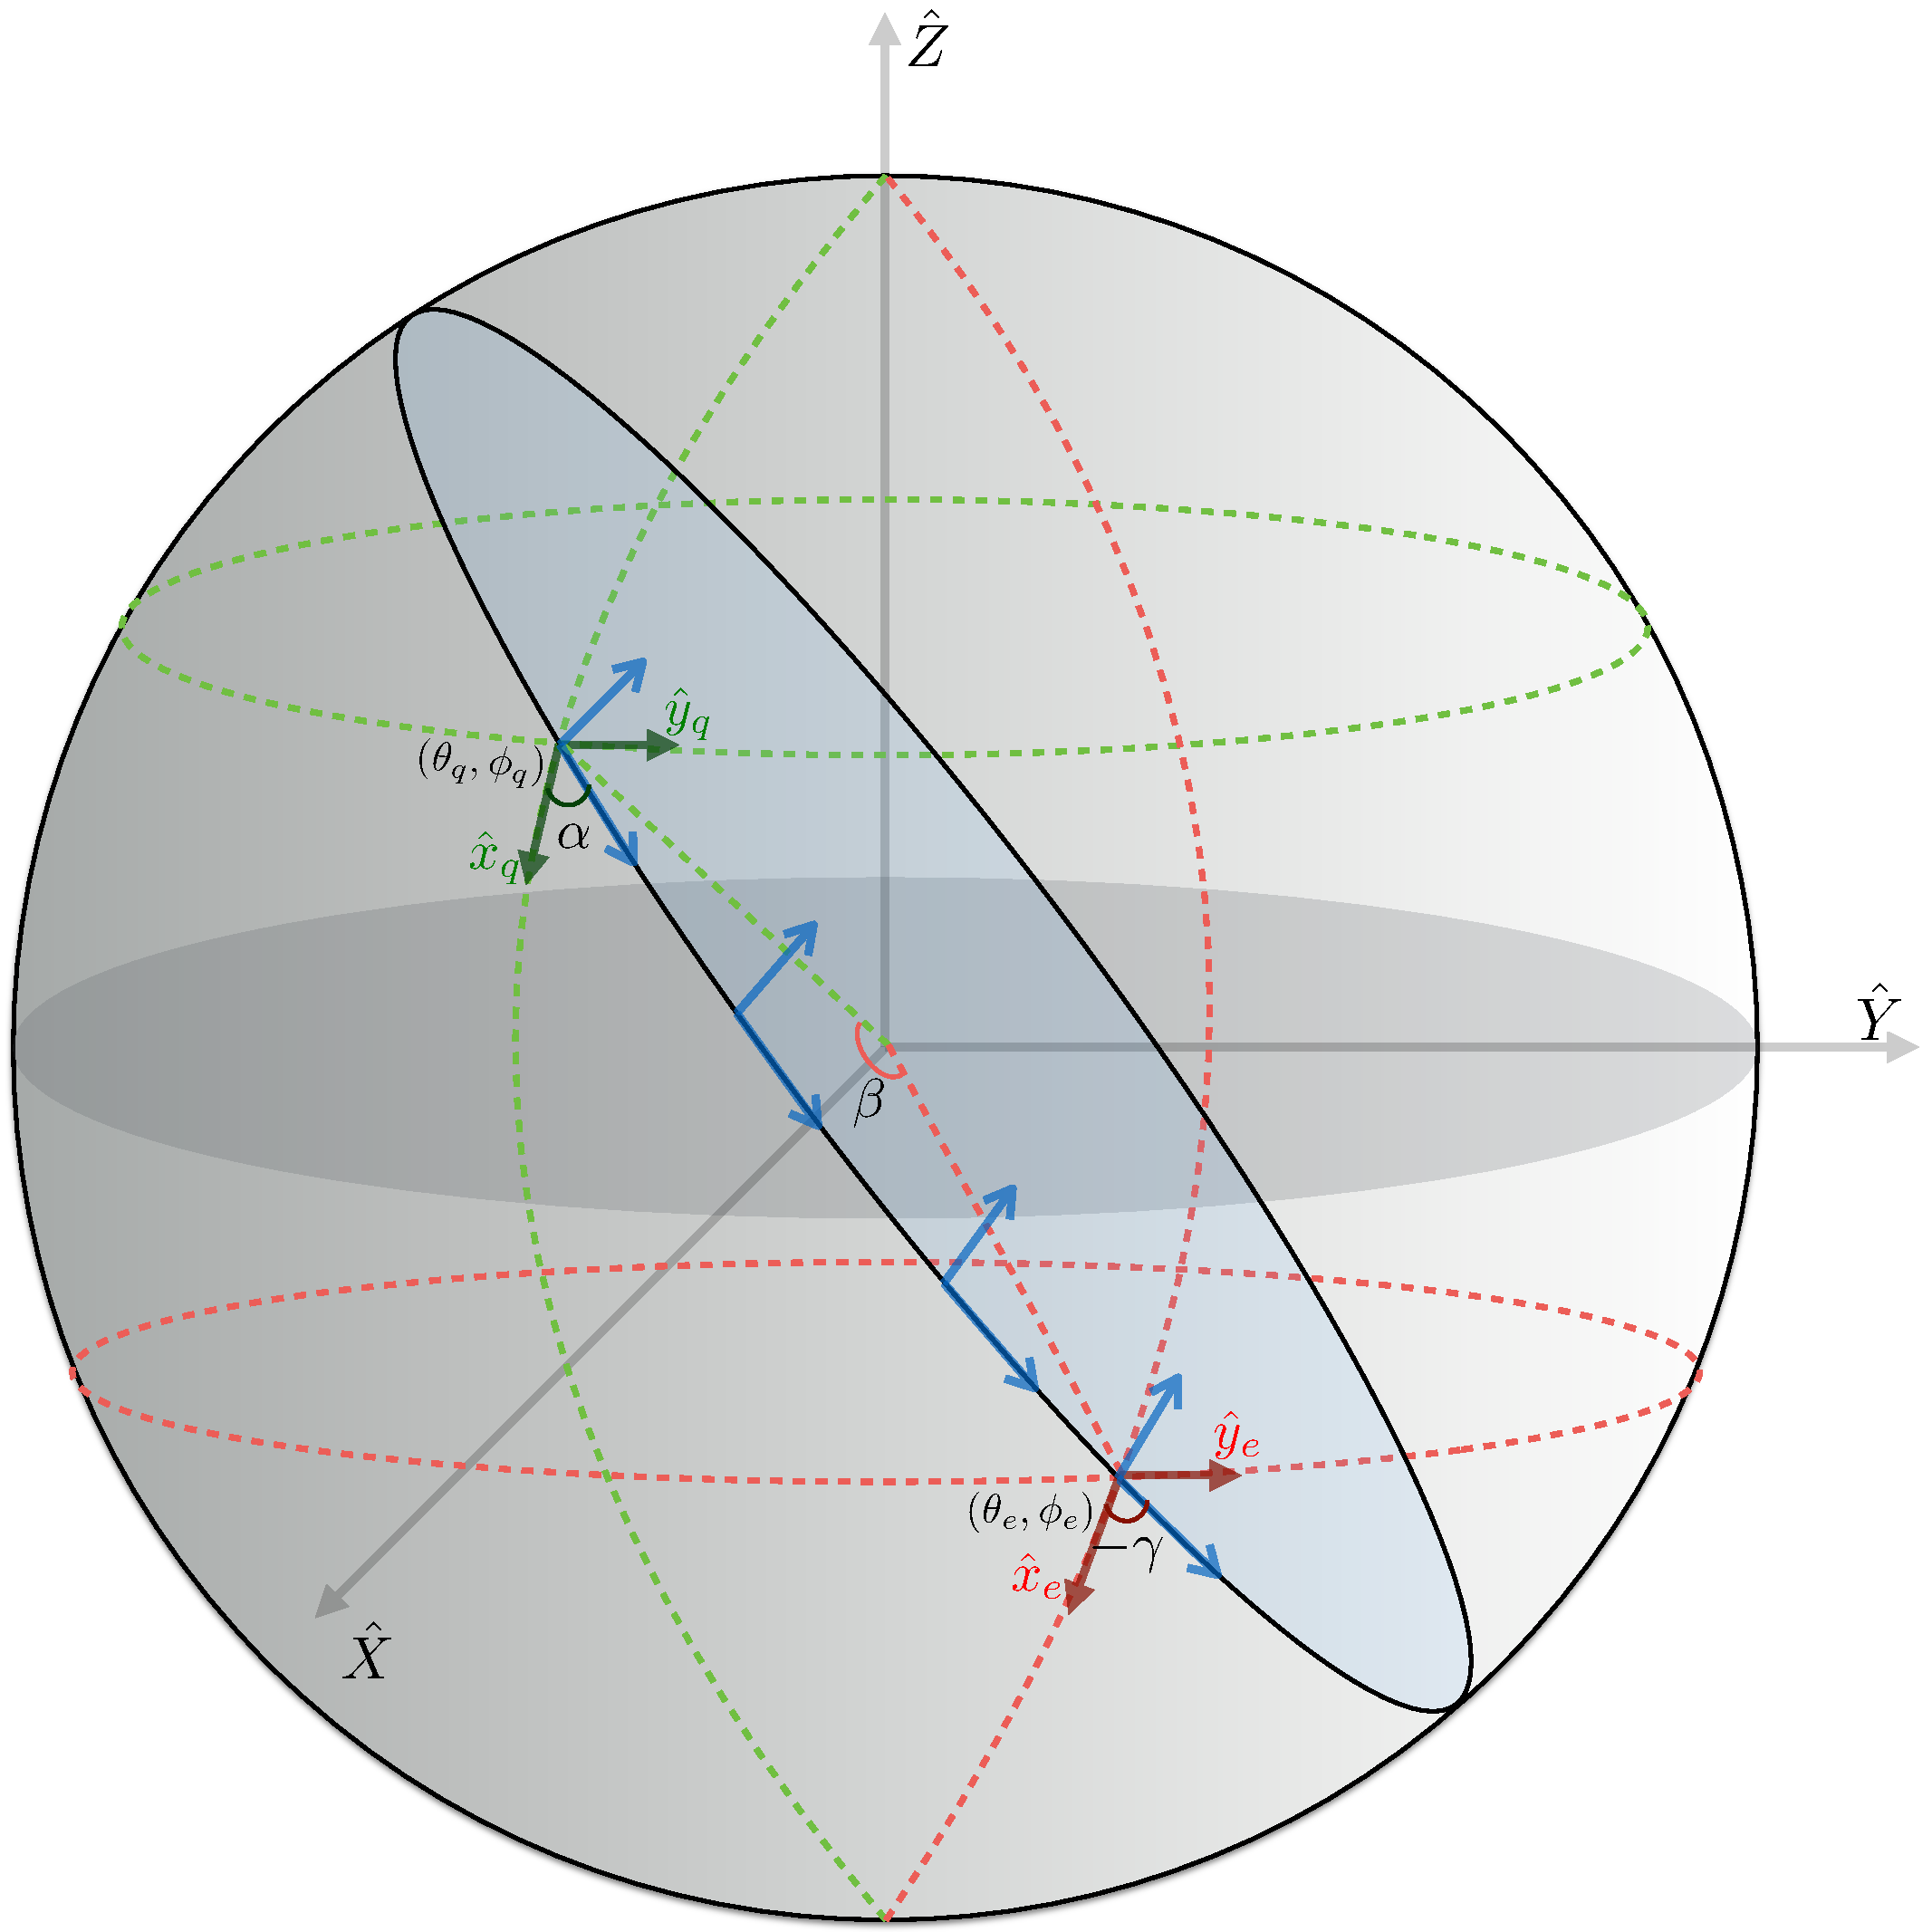
\includegraphics[width=0.5\columnwidth]{euler.pdf}
\caption{This figure depicts the Euler angles in the z-y1-z2 convention. The cartesian coordinates shown in dark green are those that lie in the tangent plane at location $\hat{n}_q = (\theta_q, \phi_q)$ while those shown in dark red are the ones that lie in the tangent plane at location $\hat{n}_e = (\theta_e, \phi_e)$. The blue coordinates at different locations are representative of the parallel transport along the geodesic connection the two locations $\hat{n}_q$ \& $\hat{n}_e$ on the sphere.}
\label{fig:euler_angles}
\end{figure}
%
 
Rotating the cartesian coordinates in the tangent plane at location $\hat{n}_q$ by an angle $\phi$ about the local $\hat{z}_q$ axis, the Stokes parameters in the new coordinate system relate to those in the original coordinate system as:
$\mathcal{R}_{\hat{z}_q}(\phi)[{}_{+2}X(\hat{n}_q)] =  {}_{+2}X(\hat{n}_q) e^{-i2\phi} $.
This same rotation by $\phi$ alters the Euler angle $\alpha_{qe}$ (that aligns the $x$-axis at $\hat{n}_q$ along the geodesic to the location $\hat{n}_e$): $\mathcal{R}_{\hat{z}_q}(\phi)[\alpha_{qe}] = \alpha_{qe} - \phi$.  Therefore one can see that $\mathcal{R}_{\hat{z}_q}(\phi)[e^{-i2\alpha_{qe}}] =  e^{-i2\alpha_{qe}} e^{i2\phi}$.

Given these transformation properties, the combination ${}_{+2}X(\hat{n}_q)e^{-i2\alpha_{qe}}$ is invariant under rotations and must be spin-0 by definition:
\beq
\mathcal{R}_{\hat{z}_q}(\phi)[{}_{+2}X(\hat{n}_q)e^{-i2\alpha'_{qe}}] = {}_{+2}X(\hat{n}_q) e^{-i2\alpha_{qe}}
\eeq
\revisit{I'm having some trouble understanding the next 2 sentences.} The real part of the function is constructed by product of functions $(Q\cos{2\alpha}, U\sin{2 \alpha})$ having the same parity and hence the real part must have even parity.  At the same time, the imaginary part of the function is constructed by multiplying functions $(Q\sin{2 \alpha}, U\cos{2\alpha})$ of opposite parity and hence must have an odd parity. Therefore we can make the association that contributions to  $(E+iB)(\hat n_e)$ must be proportional to $ {}_{+2}X(\hat{n}_q) e^{-i2\alpha_{qe}}$.


The same rotation $\mathcal{R}_{\hat{z}_q}(\phi)$ leaves the Euler angle $|\beta_{qe}|$ unaltered (it measures the angular distance between the points).  Thus we can conclude that the contribution to $(E+iB)(\hat n_e)$ from the position $n_q$ must have the form 
\beq
{}_{+2}X(\hat{n}_q) f(\beta_{qe})  e^{-i2\alpha_{qe}}
\eeq
for some real function $f$.  Note that when the two locations coincide ($\beta_{qe}=0$) then  $\alpha_{qe}=0,2\pi,4\pi,\dots$, implying $E + iB \propto Q+iU$.  This is a contradiction because $Q+iU$ does not transform as a spin-0 field under local rotations, and so we must have $f(\beta_{qe} = 0 ) = 0$.   Hence the $E/B$ fields are necessarily non-local.  A similar contradiction arises when the two locations are diametrically opposite, $\beta_{qe} = \pi$, and so $f(\beta_{qe} = \pi ) = 0$.  Any such function $f$ will let us construct $E/B$-like scalar fields.  Below we derive the particular one that gives rise to our familiar $E/B$ modes.

This type of real-space construction can be generalized to transform a field of any spin to a field of any other spin, not just two and zero, and so we can use a similar construction (in the opposite direction) to transform $E/B$ maps back to the Stokes parameters (i.e. transforming spin-0 fields to spin-2).

%--------------------------------------------------------
\subsection{Standard $E$/$B$ fields}


The standard construction of $E/B$ fields depend on the spin-raising and -lowering operators, and is usually carried out in harmonic space.  The spin-raising operator ($\eth$), applied to a field of spin-s $_{s}g$, results in a fields with spin-$(s+1)$: $(\eth _{s}g)' = e^{-i(s+1)\phi}(\eth _{s}g)$  \cite{goldberg67}.  The complementary spin-lowering operator $(\bar{\eth})$  similarly results with $(\bar{\eth} _{s}g)' = e^{-i(s-1)\phi}(\bar{\eth} _{s}g)$.  The complex spin-0 scalar now arise from  the spin-2 fields ${_{\pm 2}X}$ as follows,
%
\begin{subequations}\label{eq:ebdef}
\beqry
\mathcal{E}(\hat{n}) + i \mathcal{B}(\hat{n}) &=& -\bar{\eth}^2 _{+ 2}\bar{X}(\hat{n}) \,,\label{eq:ebdef_lower}\\
\mathcal{E}(\hat{n}) - i \mathcal{B}(\hat{n}) &=& -{\eth}^2 _{-2}\bar{X}(\hat{n}) \,.
\eeqry
\end{subequations}
%
%which by the virtue of being scalars are independent of coordinate definitions. %The real part of this complex spin-0 scalar field corresponds to the E-mode while the imaginary part to the B-modes \cite{Kamionkowski1997}. 
The $\cal E/B$ fields are defined locally at point $\hat n$ in terms of the derivative operators $\eth$ and $\bar \eth$.

We can decompose the complex field $_{\pm 2}X$ into spin spherical harmonic functions: ${}_{\pm 2}X(\hat{n}) = \sum_{\ell m} {}_{\pm 2} X_{\ell m} {}_{\pm 2}Y_{\ell m}(\hat{n})$. On applying the spin raising and lowering operators on the spin spherical harmonic functions leads to the following identities \cite{goldberg67},
%
\begin{subequations}\label{eq:spinopylm} 
\beqry
\eth _s Y_{lm}(\hat{n}) &=& \sqrt{(\ell-s)(\ell+s+1)} _{s+1} Y_{lm}(\hat{n}) \,, \\
\bar{\eth} _s Y_{lm}(\hat{n}) &=& -\sqrt{(\ell+s)(\ell-s+1)} _{s-1} Y_{lm}(\hat{n}) \,, 
\eeqry
\end{subequations}
%
where $_s Y_{lm}(\hat{n}) $ denote the spin-s spherical harmonics.

From the definition of $\mathcal{E/B}$, the spin spherical harmonic decomposition of ${}_{\pm2}X$, and the identities given in \eq{eq:spinopylm}, it follows that the scalar fields $\mathcal{E}/\mathcal{B}$ are,
%
\beq \label{eq:pseudo}
\mathcal{E}(\hat{n}) = \sum_{\ell m} a^{E}_{\ell m} \sqrt{\frac{(\ell+2)!}{(\ell-2)!}} Y_{\ell m} (\hat{n});\qquad
\mathcal{B}(\hat{n})  =\sum_{\ell m} a^{B}_{\ell m} \sqrt{\frac{(\ell+2)!}{(\ell-2)!}} Y_{\ell m} (\hat{n}) \,,
\eeq
%
where the harmonic coefficients $a^{E}_{\ell m}$ and  $a^{B}_{\ell m}$ relate to the harmonic coefficients of the spin-2 polarization field via,
%
\beq\label{eq:x2eb}
a^{E}_{\ell m} = -\frac{1}{2} \Big[ {}_{+2}\tilde{X}_{\ell m} + {}_{-2}\tilde{X}_{\ell m} \Big];\qquad a^{B}_{\ell m} = -\frac{1}{2i} \Big[ {}_{+2}\tilde{X}_{\ell m} - {}_{-2}\tilde{X}_{\ell m} \Big] \,.
\eeq
%
In the remainder of this article, we will work with the scalar $E$ and pseudo scalar $B$ fields, defined by: 
%
\beq \label{eq:realeb}
E(\hat{n}) = \sum_{\ell m} a^{E}_{\ell m} Y_{\ell m} (\hat{n});\qquad B(\hat{n})  =\sum_{\ell m} a^{B}_{\ell m} Y_{\ell m} (\hat{n}) \,.
\eeq
%
These $E/B$ fields are merely red-filtered versions of $\mathcal{E}/\mathcal{B}$ (their spherical harmonic coefficients of expansion are related by the factor $[{(\ell+2)!}/{(\ell-2)!}]^{1/2}$), and are not local functions of Stokes $Q/U$. %We make this choice since the CMB spectra are more closely related to the fields E \& B.







\section{Real space polarization operators}
\subsection{Matrix notation} \label{sec:mat_pol_intro}
Our derivation of real space operators is more transparent in a matrix-vector notation.\footnote{While we work with the matrix and vector sizes given in terms of some pixelization parameter $\rm N_{\rm pix}$, all the relations are equally valid in the continuum limit attained by allowing $\rm N_{\rm pix}\rightarrow \infty$}
We introduce a matrix that encodes spin spherical harmonic basis vectors,
%
\beq
{}_{|s|}\mathcal{Y}= \bmat _{+s}Y & 0 \\ 0 & _{-s}Y \emat _{2 \rm N_{\rm pix} \times 2 \rm N_{\rm alms}} \,%,
\eeq
%
%where $s$ denotes the spin of the basis functions.
We will be working with cases $s \in [0,2]$. Each column maps to a specific harmonic basis function (i.e. indexed by $\ell m$) and each row maps to a pixel on the sphere. This matrix is not square in general: the number of rows is determined by the pixelization and the number of columns is set by the number of basis functions (e.g. determined by the band limit).

We now define the different polarization data vectors and their representation in real  space as and harmonic as follows,\footnote{We adopt a convention in which real space quantities are denoted by bar-ed variable while those in harmonic space are denoted by tilde-ed variables.}
%
\beqrys
\bar{S} &=& \bmat E \\ B  \emat_{2 \rm N_{\rm pix} \times 1} ~~~~;~~ \bar{X} = \bmat _{+2}X \\ _{-2}X \emat_{2 \rm N_{\rm pix} \times 1} ~~;~~\bar{P} =\fqu_{\tiny {2 \rm N_{\rm pix} \times 1}} \,, \\
\tilde{S} &=& \bmat a^{E} \\ a^{B} \emat _{2 \rm N_{\rm alms} \times 1}  ~~; ~~ \tilde{X} = \bmat _{+2} \tilde{X} \\ _{-2} \tilde{X} \emat_{2 \rm N_{\rm alms} \times 1} \,.
\eeqrys
%
The different symbols have the same meaning as that discussed in \sec{sec:pol-primer}, except that the subscript ${\ell m}$ for the spherical harmonic coefficients is suppressed for cleaner notation.

We define transformations between different representations of the polarization field (i.e. from $Q,U$ to $_{\pm2} X$):
%
\beqrys
\bar T &=& \qutox_{2 \rm N_{\rm pix} \times 2 \rm N_{\rm pix}} ~~;~~ \bar T^{-1} = \frac{1}{2} \bar T^{\dagger} \,, \\
\tilde T &=& -\qutox_{2 \rm N_{\rm alms} \times 2 \rm N_{\rm alms}} ~~;~~ \tilde T^{-1} = \frac{1}{2} \tilde T^{\dagger} \,,
\eeqrys
%
The sign conventions we have chosen match HEALPix.
Using the data vectors and the matrix operators defined above we can now express, in compact notation, the forward and inverse relations between different representations of the polarization data vectors as follows,
%
\begin{subequations} \label{eq:pol_data_relns}
  %Kevin's version
  \beqry
  \bar{X} &= \bar T  \bar{P}; &\qquad \bar{P} = \frac{1}{2} \bar T^{\dagger}  \bar{X} ; \\
  \tilde{X} &= \tilde T \tilde{S}; &\qquad \tilde{S} = \frac{1}{2}\tilde T^{\dagger} \tilde{X} \,.
  \eeqry
  Meanwhile the spherical harmonic transforms are written as:
  \beqry
  \bar X &=  {{}_2\mathcal{Y}}  \tilde X; &\qquad \tilde X ={{}_2\mathcal{Y}}^{\dagger}  \bar X  ; \\
  \bar S &=  {{}_0\mathcal{Y}} \tilde S; &\qquad  \tilde S =  {{}_0\mathcal{Y}}^{\dagger} \bar S \,.
  \eeqry
% Aditya's version
%\beqry
%\bar{X} &=& \bar T * \bar{P} ~~;~~\bar{P} = \frac{1}{2} \bar T^{\dagger} * \bar{X} \,, \\
%\bar X &=&  {{}_2\mathcal{Y}} * \tilde X  ~~;~~ \tilde X ={{}_2\mathcal{Y}}^{\dagger} * \bar X  \,, \\
%\tilde{X} &=& \tilde T * \tilde{S} ~~;~~ \tilde{S} = \frac{1}{2}\tilde T^{\dagger} * \tilde{X} \,.\\ 
%\bar S &=&  {{}_0\mathcal{Y}} * \tilde S ~~;~~  \tilde S =  {{}_0\mathcal{Y}}^{\dagger} * \bar S \,.
%\tilde X &=&  {{}_2\mathcal{Y}}^{\dagger} * \bar X ~~;~~ \tilde{X} = \tilde T * \tilde{S} \,, \\
%\bar{S} &=& {{}_0\mathcal{Y}}*\tilde S ~~;~~ \tilde{S} = \frac{1}{2}\tilde T^{\dagger} * \tilde{X} \,.\\
%\bar{X} &=& \bar T * \bar{P} ~~;~~ \tilde{X} = \tilde T * \tilde{S} \,, \\
%\bar{P} &=& \frac{1}{2} \bar T^{\dagger} * \bar{X} ~~;~~ \tilde{S} = \frac{1}{2}\tilde T^{\dagger} * \tilde{X} \,. \\
%\eeqry
\end{subequations}
%
Finally we introduce the operators that project harmonic space data vector to the $E$ or $B$ subspace,
%
\begin{subequations} \label{eq:har_eb_op}
\beqry
\tilde O_E &=& \bmat \mathbb{1} & \mathbb{0} \\ \mathbb{0} & \mathbb{0} \emat _{2 \rm N_{\rm alms} \times 2 \rm N_{\rm alms} }   ~~;~~ \tilde S_E = \tilde O_E  \tilde S ,\\
\tilde O_B &=& \bmat \mathbb{0} & \mathbb{0} \\ \mathbb{0} & \mathbb{1} \emat _{2 \rm N_{\rm alms} \times 2 \rm N_{\rm alms} } ~~; ~~ \tilde S_B = \tilde O_B  \tilde S .
\eeqry
\end{subequations}
%
Note that these harmonic space matrices are idempotent ($\tilde O_E  \tilde O_E = \tilde O_E;  \tilde O_B  \tilde O_B= \tilde O_B$), orthogonal ($\tilde O_E  \tilde O_B = \mathbb{0}$), and sum to the identity matrix ($\tilde O_E + \tilde O_B = \mathbb{1}$).
%
%\begin{subequations} \label{eq:har_op_prop}
%\beqry
%\tilde O_E  \tilde O_E&=& \tilde O_E ~~;~~  \tilde O_B  \tilde O_B= \tilde O_B \,,\\
% \tilde O_E  \tilde O_B&=& \mathbb{0} \,, \label{eq:op_eb_ortho}\\ 
% \tilde O_E + \tilde O_B&=& \mathbb{1} \,.
%\eeqry
%\end{subequations}
%
The above relations for these harmonic space operators are exactly valid.  In the following sections we aim to derive the real space analogues ($O_E,O_B$) of these harmonic space operators.



\subsection{Evaluating scalar $E/B$ from Stokes $Q/U$}\label{sec:qu2eb}
In \sec{sec:pol-primer} we described the conventional procedure of computing the scalar fields $E/B$ from the Stokes parameters $Q/U$. 
%To reiterate, this process involved taking the spin harmonic transform of the complex spin-2 fields ${}_{\pm2} \bar X$, forming specific linear combinations of the resultant coefficients of expansion ${}_{\pm 2} \tilde X_{\ell m}$ and evaluating the forward spin-0 transform to derive the scalar E \& B fields. 
In this section we derive the real space convolution kernels on the sphere which can be used to directly evaluate the scalar fields $E$ \& $B$ on the sphere.  We use the vector-matrix notation introduced in \sec{sec:mat_pol_intro} to write down an operator equation relating the real space vector of scalars \vs to the Stokes polarization vector \vp{},
%
\beqrys
\bar{S} &=& {{}_0\mathcal{Y}} \, \tilde T^{-1}  \, {{}_2\mathcal{Y}^{\dagger}} \, \bar T  \bar{P}
= \frac{1}{2} {{}_0\mathcal{Y}} \, \tilde T^{\dagger} {{}_2\mathcal{Y}^{\dagger}} \, \bar T \bar{P}    \\
&=&  \bar O \bar{P}. \label{eq:qu2eb_op}
\eeqrys
%
The explicit form of the real space operator $\bar O$ can be derived by contracting over all the matrix operators. This procedure is explicitly worked out in the following set of equations,
%
\beqrys
\bar{O} &=& \frac{1}{2} {{}_0\mathcal{Y}}\, \tilde T^{\dagger} {{}_2\mathcal{Y}^{\dagger}} \, \bar T \,, \\
&=& -0.5 \yzmat{e} \qutoxd \ymatc{q} \qutox   \,, \\
&=& -0.5 \begin{bmatrix} \sum ({}_{0}Y_e ~{}_{2}Y^{\dag}_q  +  {}_{0}Y_e~ {}_{-2}Y^{\dag}_q) & {\rm i}  \sum ({}_{0}Y_e ~ {}_{2}Y^{\dag}_q - {}_{0}Y_e ~{}_{-2}Y^{\dag}_q)  \\  - {\rm i} \sum  ({}_{0}Y_e ~ {}_{2}Y^{\dag}_q - {}_{0}Y_e~ {}_{-2}Y^{\dag}_q) & \sum ({}_{0}Y_e~ {}_{2}Y^{\dag}_q + {}_{0}Y_e ~{}_{-2}Y^{\dag}_q)  \end{bmatrix} \,, \label{eq:qu2eb_ker_1}
\eeqrys
%
where the symbol ${}_{0}Y_e$ is used to denote the sub-matrix ${}_{0}Y_{\hat{n}_e \times \ell m} \equiv {}_{0}Y_{\ell m}(\hat{n}_e)$, the symbol ${}_{\pm 2}Y^{\dag}_q$ is used to denote the transposed conjugated matrix ${}_{\pm 2}Y^*_{\ell m \times \hat{n}_q} \equiv {}_{\pm 2}Y^*_{\ell m}(\hat{n}_q)$ and the summation is over the multipole indices $\ell,m$. As before, we use the notation that the index $e$ denotes the location where the scalar fields are being evaluated, and the index $q$ denotes the location from which  the Stokes parameters are being accessed. Using the conjugation properties of the spin spherical harmonic functions it can be shown that the following identity holds true,
%
\beq
 \left [\sum_{\ell m} {}_{0}Y_{\ell m}(\hat{n}_e){}_{+2}Y^*_{\ell m}(\hat{n}_q)\right]^* = \sum_{\ell m} {}_{0}Y_{\ell m}(\hat{n}_e){}_{-2}Y^*_{\ell m}(\hat{n}_q) \,,
 \eeq
 %
where the terms on either side of the equation are those that appear in \eq{eq:qu2eb_ker_1}. Note that the operator $\bar{O}$ is real as one expects, since each sub-matrix in \eq{eq:qu2eb_ker_1} is formed by summing a complex number and its conjugate. 

\noindent \eq{eq:qu2eb_ker_1} already presents a real space operator, but it is not in a form which can be practically implemented. To proceed, we use the fact that the $m$ sum over the product of two spin spherical harmonic functions can be expressed as a function of the Euler angles \cite{varshalovich},
%
\beq \label{eq:sum_spin_shf}
 \sum_{m}{{}_{s_1}Y}^*_{\ell m}(\hat{n}_i)\,{{}_{s_2}Y}_{\ell m}(\hat{n}_j) = \sqrt{\frac{2\ell+1}{4 \pi}} {{}_{s_2}}Y_{\ell \,-s_1}(\beta_{ij},\alpha_{ij}) e^{- i s_2 \gamma_{ij}} \,,
\eeq
%
where $\alpha_{ij}, ~\beta_{ij} ~\&~ \gamma_{ij}$ denote the Euler angles that specifically transform $(i \rightarrow j)$: the coordinate system at $\hat{n}_i$ to align the coordinate system at $\hat{n}_j$\footnote{The sense of the rotation become more obvious when this equation is written in terms of the Wigner-D functions.}.

Using this identity, the different parts of the real space operator $\bar{O}$  (from eq.~\ref{eq:qu2eb_ker_1}) are completely specified by the complex function,
%
\begin{subequations}\label{eq:qu2eb_gen_kernel}
\beqry
\mathcal{M}( \hat{n}_e, \hat{n}_q)  &=& \mathcal{M}_{r} + i \mathcal{M}_{i}  \,,\nonumber \\ 
&=&\sum_{\ell m} {{_0}Y}_{\ell m}(\hat n_e) \, {{_{-2}}Y}^*_{\ell m}(\hat n_q) = \sum_{\ell} \sqrt{\frac{2\ell+1}{ 4 \pi}}{{_0Y}_{\ell 2}}(\beta_{qe},\alpha_{qe})\,,\\
&=&  \Big [ \cos(2 \alpha_{qe}) + i \sin(2 \alpha_{qe} ) \Big]   \sum_{\ell=\ell_{\rm min}}^{\ell_{\rm max}} {\frac{2\ell+1}{ 4 \pi}} \sqrt{\frac{(\ell-2)!}{(\ell+2)!}}P_{\ell 2} (\cos\beta_{qe}) \,, \label{eq:rad_ker_queb} \\
&=&  \Big [ \cos(2 \alpha_{qe}) + i \sin(2 \alpha_{qe} ) \Big] \quad {{}_{\mm}f}(\beta_{qe},\ell_{\rm min},\ell_{\rm max}) \,, 
\eeqry
\end{subequations}
%
where we have used the identity in \eq{eq:sum_spin_shf} to simplify the product of the spherical harmonic functions. Note that the function depends only on two out of the three Euler angles.  The azimuthal part depends only on the Euler angle $\alpha_{qe}$, and so its harmonic transform has no multipole $\ell$ dependence.  The azimuthal part is the crucial operation that translates between different spin representation of CMB polarization. Only the radial part $f(\beta_{qe})$ depends only on the angular separation between locations and hence  completely incorporates all the multipole $\ell$ dependence. 

Employing \eq{eq:qu2eb_gen_kernel} to simplify the product of spherical harmonic functions in \eq{eq:qu2eb_ker_1}, the real space operator $\bar{O}$ can now be cast in this more useful form,
%
\beq\label{eq:op_qu2eb_rad}
\bar O =-\bmat  \mathcal{M}_{r} & \mathcal{M}_{i} \\  -\mathcal{M}_{i}  & \mathcal{M}_{r} \emat_{2 N_{\rm pix} \times 2 N_{pix}} = -{{}_{\mm}f}(\beta_{qe},\ell_{\rm min},\ell_{\rm max})\bmat \cos(2 \alpha_{qe}) & \sin(2\alpha_{qe})\\  -\sin(2 \alpha_{qe})  & \cos(2 \alpha_{qe}) \emat \,,
\eeq
%
where $(\alpha_{qe}, ~\beta_{qe}, \gamma_{qe})$ denote the Euler angles which rotate the local cartesian system at $\hat{n}_q$ (location where Stokes parameters are accessed) to the cartesian system at  $\hat{n}_e$ (location where the scalar fields are evaluated): $\mathcal{R}(\alpha_{qe},\beta_{qe},\gamma_{qe})[\hat{n}_q] = \hat{n}_e$. 



\paragraph{Radiation kernel.} The expression we call the \textit{radiation kernel}  allows us, like a Green's function, to evaluate the $E/B$ field contribution due to a single Stoke parameter ``charge'' at a fixed location. The total $E/B$ maps can then be thought of as the superposed radiation emerging from Stokes charges across the sphere. In this picture, we are effectively in the frame of the Stokes charge ${}_{\pm2}X$ and evaluate its contribution to the complex spin-0 scalar field $E+iB$ across the sphere.

The $E$/$B$ contribution from the Stokes parameters at some location $\hat{n}_q$ is given by the following expression (\eq{eq:op_qu2eb_rad} and \eq{eq:qu2eb_op}),
%
\beq  \label{eq:qu2eb_radiation_explicit}
\bar{S}_q(\hat n_e) = \bmat E_e \\ B_e  \emat_{q} =- {{}_{\mm}f}(\beta_{qe},\ell_{\rm min},\ell_{\rm max})\bmat \cos(2 \alpha_{q e}) & \sin(2\alpha_{q e})\\  -\sin(2 \alpha_{q e})  & \cos(2 \alpha_{q e}) \emat  \bmat Q_{q} \\ U_{q}  \emat \Delta \Omega \,.
\eeq
%
The total map can be simply evaluated by summing over the contribution from the Stokes parameters at each location $\hat{n}_q$: $\bar{S} = \sum_{q=1}^{N_{\rm pix}} \bar{S}_q$. This operation can be cast concisely as,
%
\begin{subequations} \label{eq:qu2eb_radiation_concise}
\beqry 
\left[E + iB\right](\hat{n}_e) &=& -\Delta \Omega  \sum_{q=1}^{N_{\rm pix}} \Big[ {}_{+2}X(\hat{n}_{q}) e^{-i2\alpha_{q e}} \Big]  {{}_{\mm}f}(\beta_{q e}) \,, \\
%&=&    \sum_{q=1}^{N_{\rm pix}} \Bigg\lbrace {}_{+2}X(\hat{n}_{q}) \left[ - \Delta \Omega \sum_{\ell=\ell_{\rm min}}^{\ell_{\rm max}} \sqrt{\frac{2 \ell+1}{4 \pi}}Y^*_{\ell 2}(\beta_{qe},\alpha_{qe}) \right] \Bigg\rbrace \,, \\
&=& \sum_{q=1}^{N_{\rm pix}} {}_{+2}X(\hat{n}_{q}) \,  \mathcal{M}_{G}(\hat n_e,\hat{n}_q) \,,
\eeqry
\end{subequations}
%
where the last line is a simple scalar multiplication between complex numbers.  The radiation kernel is then:
\beq
 \mathcal{M}_{G}(\hat{n}_e,\hat n_q) =  - \Delta \Omega {{}_{\mm}f}(\beta_{qe},\ell_{\rm min},\ell_{\rm max}) e^{-i2\alpha_{q e}}
\eeq
%. $\mathcal{M}_{G}$ is merely the conjugated function $\mm^*$ when expressed as a function of the Euler angle $\alpha_{qe}$ and it
is $-\Delta\Omega \mm^*$ and can be thought of as the Green's function of the operator.  That is, $[E +iB](\hat n_e) = \mathcal{M}_{G}(\hat n_e,\hat n_q)$ is the spin-0 scalar field generated from the delta-function Stokes field $[Q+iU](\hat n) = [\delta(\hat{n}-\hat{n}_q) + i0]$. We display the kernel later in \fig{fig:vis_kernel}.
 

%
\begin{figure}[!t]
\centering
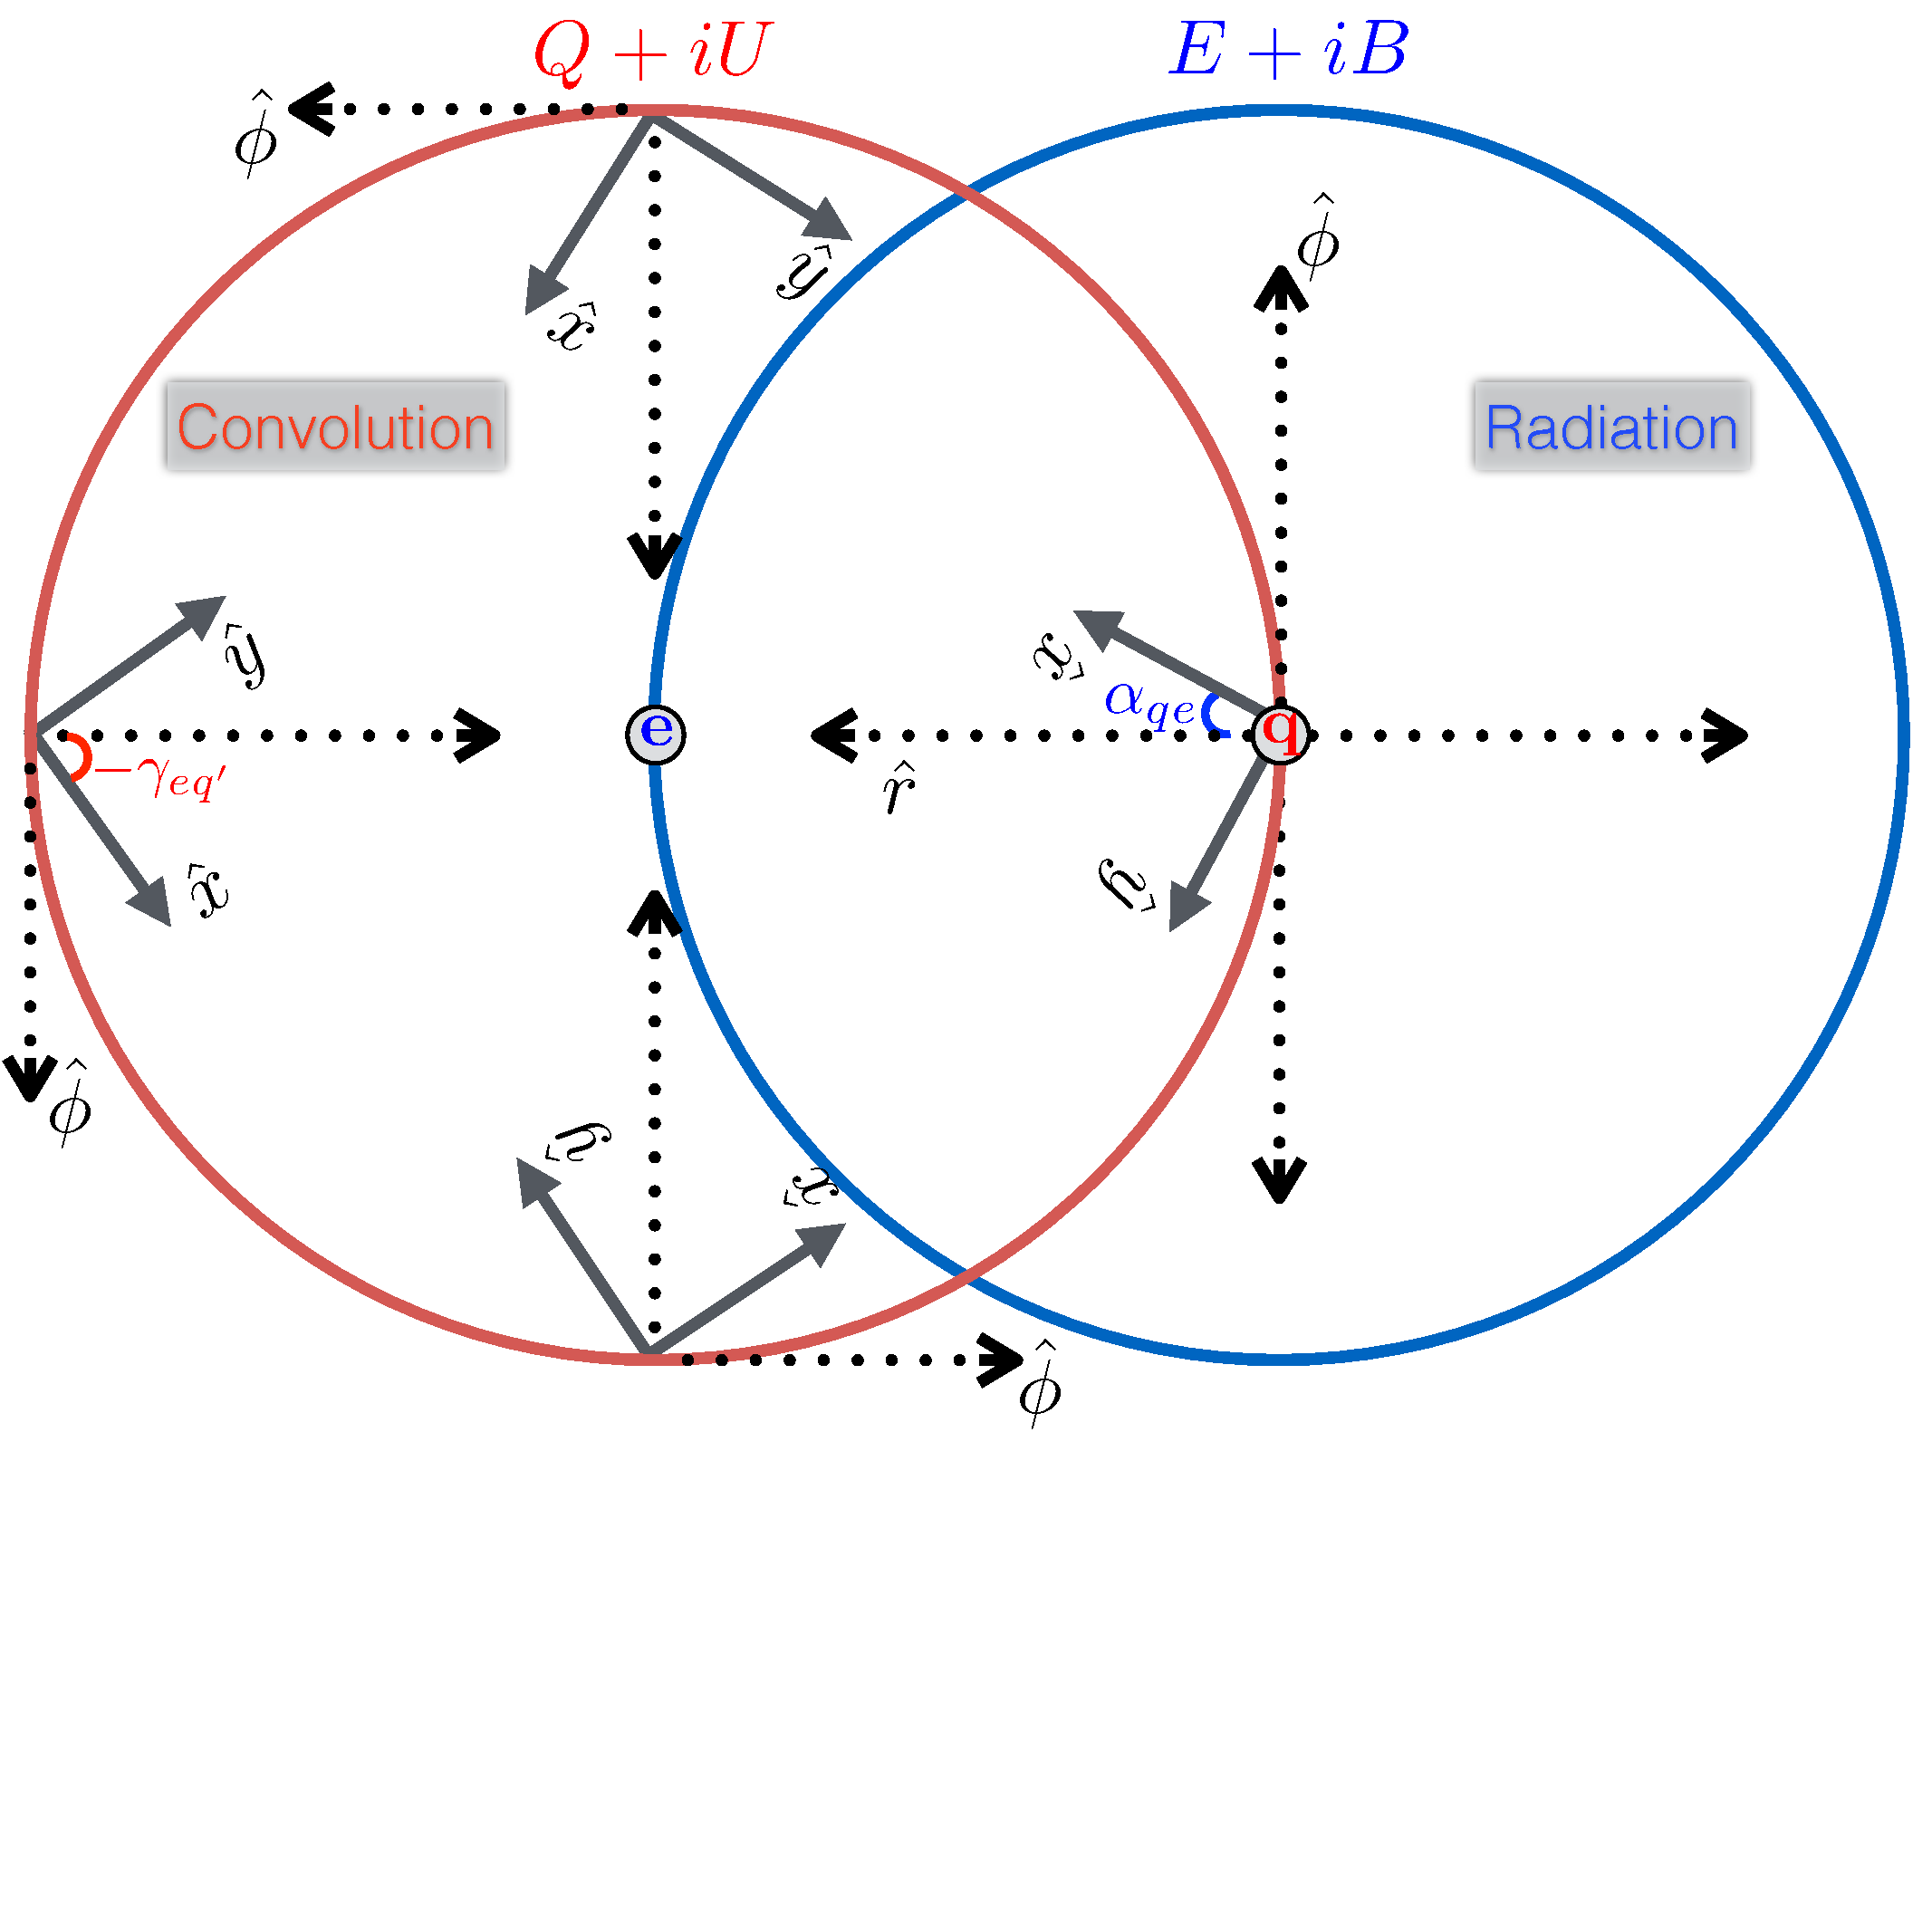
\includegraphics[width=0.5\columnwidth]{radiation_convolution.pdf}
\caption{The local cartesian coordinate are only drawn on the red circle, representative of the coordinate dependence of the Stokes parameters. The value of the scalar field at location `e' can be evaluated by summing over the contribution from all the Stokes parameters on the red circle (sphere). The convolutions are performed with kernels which are defined in term of the Euler angle $\gamma_{eq}$. Alternatively, one can compute the contribution from the Stokes parameter at location `q' to all the point on the blue circle(sphere) and this is a function of the Euler angle $\alpha_{eq}$. In the flat sky limit, since $\gamma=-\alpha$ there is no difference between the radiating and convolving kernels.}
\label{fig:planar_euler_angles}
\end{figure}
%

\paragraph{Convolution kernel.} We can also formulate the real space operator as a convolution operation, where the scalar field at $\hat n_e$ gathers contributions from the Stokes fields.  This is based around the inverse rotation from the previous section (to align the coordinate system at $\hat{n}_e$ with that at $\hat{n}_q$).  The inverse rotation Euler angles relates to the forward rotation Euler angles by the following relations: $\alpha_{eq}=-\gamma_{qe}$, $\beta_{eq} = -\beta_{qe}$ and  $\gamma_{eq} =-\alpha_{qe}$. Since the kernel only depends on the cosine of the Euler angle $\beta$, it is immune to changes in its sign. The operator equation can be expressed as a function of the Euler angle $\gamma_{eq}$ as follows, 
%
\beq \label{eq:qu2eb_convolution_explicit}
\bmat E_e \\ B_e  \emat =- \sum_{q=1}^{N_{\rm pix}}{{}_{\mm}f}(\beta_{eq},\ell_{\rm min},\ell_{\rm max})\bmat \cos(2 \gamma_{eq}) & -\sin(2\gamma_{eq})\\  \sin(2 \gamma_{eq})  & \cos(2 \gamma_{eq}) \emat  \bmat Q_q \\ U_q  \emat \Delta \Omega\,,
\eeq
%
%where $\Delta \Omega$ denotes the pixel area and all the symbols have their usual meaning. 
\revisit{This version of the real space operator would have naturally emerged had we simplified the the equivalent function $\sum_{\ell m} {}_{0}Y^*_{\ell m}(\hat{n}_e){}_{+2}Y_{\ell m}(\hat{n}_q)$ in \eq{eq:qu2eb_gen_kernel}.} This formulation of the real space operator can be interpreted as integrating at some fixed location $\hat{n}_e$ the $E/B$ mode contribution arising from the Stokes parameters at all location $\hat{n}_q$ on the sphere. This operation can be expressed more concisely as follows,
%
\begin{subequations} \label{q:qu2eb_convolution_concise}
\beqry 
[E + iB](\hat{n}_e) &=& - \Delta \Omega \sum_{q=1}^{N_{\rm pix}} \left(\sum_{\ell=\ell_{\rm min}}^{\ell_{\rm max}} \frac{2 \ell+1}{4 \pi} \sqrt{\frac{(\ell-2)!}{(\ell+2)!}} P_{\ell}^{2}(\beta_{eq}) \right) {\Bigg( e^{i2 \gamma_{eq}}   {}_{+2}X (\hat{n}_q) \Bigg)}, \label{eq:qu2eb_physical}\\
&=& \Bigg\lbrace \left[ - \Delta \Omega \sum_{\ell=\ell_{\rm min}}^{\ell_{\rm max}} \sqrt{\frac{2 \ell+1}{4 \pi}}Y_{\ell 2}(\beta_{eq},\gamma_{eq}) \right]  \star {}_{+2}X \Bigg\rbrace(\hat{n}_e) \,, \\
&=& \Bigg\lbrace \mathcal{M}_{B} \star {}_{+2}X \Bigg\rbrace(\hat{n}_e) \,, \label{eq:qu2eb_convolution} 
\eeqry
\end{subequations}
%
where $\star$ denotes a convolution and $\mathcal{M}_{B}$ is merely the conjugated function $\mm^*$.  When expressed as a function of the Euler angle $\gamma_{eq}$ it can be thought of as an effective instrument beam pointing to the direction $\hat{n}_e$.  We display the kernel in \fig{fig:vis_kernel}.
%--------------------------------------------------------

  
%--------------------------------------------------------
\subsection{Evaluating Stokes $Q$/$U$ from scalar $E$/$B$}\label{sec:eb2qu}
The real space operator which translates $E$ \& $B$ fields to Stokes parameters $Q$ \& $U$ can be derived using a similar procedure. Expressed in the matrix-vector notation, inverse operator is given by,
%
\begin{subequations}
\beqry
\bar{P} &=& \bar{T}^{-1} {{}_2\mathcal{Y}}\, \tilde T {{}_0\mathcal{Y}^{\dagger}}\bar{S} = \frac{1}{2} \bar{T}^{\dagger} {{}_2\mathcal{Y}} \,\tilde T {{}_0\mathcal{Y}^{\dagger}}\bar{S}\,,  \\
&=&  \bar O^{-1} \bar{S}\,.
\eeqry
\end{subequations}
%
%The inverse operator $\bar{O}^{-1}$ can be derived by realizing that $\mm^{-1}$ is given by the following expression,
%%
%\beq
%\mm^{-1} = \sum_{\ell m}  {{}_{2}}Y_{\ell m}(\hat n_q) {}_{0}Y^*_{\ell m}(\hat n_e) \, 
%\eeq
%%
The inverse operator expressed in terms of the function $\mm$ given in \eq{eq:qu2eb_gen_kernel} is given by the following equation,
%
\beq
{\bar O}^{-1}=-\bmat \mathcal{M}_{r} & -\mathcal{M}_{i} \\  \mathcal{M}_{i}  & \mathcal{M}_{r} \emat_{2 N_{\rm pix} \times 2 N_{pix}} =-{{}_{\mm}f}(\beta_{eq},\ell_{\rm min},\ell_{\rm max})\bmat \cos(2 \alpha_{qe}) & -\sin(2\alpha_{qe})\\  \sin(2 \alpha_{qe})  & \cos(2 \alpha_{qe}) \emat \,,
\eeq
%
where all the symbols have the same meaning as discussed in \sec{sec:qu2eb}. Note that the kernel in the above equation differs from the one in \eq{eq:op_qu2eb_rad} by a change in sign on the off-diagonals of the block matrix. When expressed in terms of the same set of Euler angles used to define the operator $\bar{O}$, it can be shown that the different forms of the real space operator are given by,
%
\beqry
    {}_{+2}X(\hat{n}_q) &=  \sum_{e=1}^{N_{\rm pix}} [E+iB](\hat{n}_{e})\   \mathcal{M}^*_{B}[\hat{n}_e] \hspace{0.8cm} &\textrm{\emph{Radiation kernel}}\,\\
    {}_{+2}X(\hat{n}_q) &= \Bigg\lbrace \mathcal{M}^*_{G} \star [E+iB] \Bigg\rbrace(\hat{n}_q) \hspace{0.8cm} &\textrm{\emph {Convolution kernel}}\,, \label{eq:eb2qu_convolution}
\eeqry
%
where all the symbols have the same meaning as defined in \sec{sec:qu2eb}. Note that the conjugated forms of the Green's function and the effective beam for the operator $\bar{O}$ have their roles reversed for the inverse operator $\bar{O}^{-1}$.
%--------------------------------------------------------

 
%--------------------------------------------------------
\subsection{Purifying Stokes parameters $Q$/$U$ for $E$/$B$ modes}
We can only measure the total Stokes vector, a sum of the part corresponding to scalar $E$ and the part corresponding to $B$.  The $E$/$B$ modes are orthogonal to each other in the sense that their respective operators are orthogonal to each other as seen in \eq{eq:op_eb_ortho}. It is possible to decompose the Stokes vector \vp{} into one \vp{\rm E} that purely contributes to $E$ modes and another \vp{\rm B} that purely contribute to the $B$ modes of polarization. In this section we derive the real space operators which operate on the total Stokes vector and yield this decomposition, without ever having to explicitly evaluate the scalar modes. The algebra is more involved, but the derivation is similar to that discussed in \sec{sec:qu2eb}, so we refrain from presenting the detailed calculations here, and outline only the key points. We use the harmonic space projection operators $\tilde O_{E/B}$, defined in \eq{eq:har_eb_op}, to derive the respective real space operators. The Stokes parameters corresponding to each scalar mode are given by the following expressions,
%
\beqry
\bar{P}_E &=&  [\bar T^{-1}  {{}_2\mathcal{Y}} \, \tilde T  \tilde O_E \tilde T^{-1}* {{}_2\mathcal{Y}^{\dagger}}\, \bar T] \bar{P}  \,, \\
&=& [\frac{1}{4} \bar T^{\dagger }  {{}_2\mathcal{Y}} \, \tilde T  \tilde O_E  \tilde T^{\dagger}  {{}_2\mathcal{Y}^{\dagger}}\, \bar T ]\bar{P}  \,, \nonumber \\
&=&  \bar O_{E} \bar{P} \,,\nonumber \\
\bar{P}_B &=&  [\bar T^{-1}  {{}_2\mathcal{Y}} \, \tilde T  \tilde O_B \tilde T^{-1} {{}_2\mathcal{Y}^{\dagger}} \bar T]\bar{P}  \,, \\
&=& [\frac{1}{4} \bar T^{\dagger }  {{}_2\mathcal{Y}}\, \tilde T  \tilde O_B \tilde T^{\dagger} {{}_2\mathcal{Y}^{\dagger}}\, \bar T] \bar{P}   \,, \nonumber\\
&=&  \bar O_{B} \bar{P} \,. \nonumber
\eeqry
%
We contract over all the matrix operators to arrive at the the real space operators. On working through the algebra it can be shown that the real space operators have the following form,
%
\beq
\bar O_{E/B} = 0.5 \bmat \mathcal{I}_{r} & \mathcal{I}_{i} \\  -\mathcal{I}_{i}  & \mathcal{I}_{r} \emat \pm 0.5 \bmat \mathcal{D}_{r} & \mathcal{D}_{i} \\  \mathcal{D}_{i}  & - \mathcal{D}_{r} \emat \,,\\
\eeq
where $\mathcal{I}_{r} ~\&~ \mathcal{D}_{r}$ and $\mathcal{I}_{i} ~\&~ \mathcal{D}_{i}$ are the real and complex parts of the following complex functions,
%
\begin{subequations}
\beqry
\mathcal{I} (\hat{n}_e,\hat{n}_q) &=& \mathcal{I}_{r} + i \mathcal{I}_{i} = \sum_{\ell m} {_{-2}Y}_{\ell m}(\hat n_e) {_{-2}Y}^*_{\ell m}(\hat n_q) \,, \\
\mathcal{D}(\hat{n}_e,\hat{n}_q)  &=& \mathcal{D}_{r} + i\mathcal{D}_{i} = \sum_{\ell m} {_2Y}_{\ell m}(\hat n_e) {_{-2}Y}^*_{\ell m}(\hat n_q) \,.
\eeqry
\end{subequations}
%
These functions can be further simplified using the identity of spin spherical harmonics given in \eq{eq:sum_spin_shf}. Specifically it can be shown that these functions reduce to the following mathematical forms,
%
\beqrys \label{eq:fn_i}
\mathcal{I}(\hat{n}_e, \hat{n}_q) &=& \sum_{\ell} \sqrt{\frac{2\ell+1}{ 4 \pi}}{_{-2}Y}_{\ell2}(\beta_{qe}, \alpha_{qe}) ~ \rm{e}^{i2 \gamma_{qe}} \label{eq:healpix-compatible-i} = \mathcal{I}_r + i \mathcal{I}_i \,, \\
\mathcal{I}_r + i \mathcal{I}_i &=& \Big [ \cos(2 \alpha_{qe} +  2\gamma_{qe}) + i \sin(2 \alpha_{qe} +  2 \gamma_{qe}) \Big]   {{}_{\mi}f}(\beta_{qe},\ell_{\rm min},\ell_{\rm max}) \,,
\eeqrys
%
%
\beqrys \label{eq:fn_d}
\mathcal{D}(\hat{n}_q, \hat{n}_e) &=& \sum_{\ell} \sqrt{\frac{2\ell+1}{ 4 \pi}}{_2Y}_{\ell 2}(\beta_{qe}, \alpha_{qe}) ~ \rm{e}^{- i2 \gamma_{qe}} \label{eq:healpix-compatible-m} =\mathcal{D}_r + i \mathcal{D}_i \,, \\
\mathcal{D}_r + i \mathcal{D}_i &=&  \Big [ \cos(2 \alpha_{qe} - 2\gamma_{qe}) + i \sin(2 \alpha_{qe} -  2 \gamma_{qe}) \Big]   {{}_{\md}f}(\beta_{qe},\ell_{\rm min},\ell_{\rm max}) \,,
\eeqrys
%
where the radial functions are given by,
%
\beq
{{}_{\mdi}f}(\beta,\ell_{\rm min},\ell_{\rm max}) = \sum_{\ell=\ell_{\rm min}}^{\ell_{\rm max}} \sqrt{\frac{2\ell+1}{ 4 \pi}} {{}_{ \mdi}f}_{\ell}(\beta) \label{eq:f2_rad_ker}\,,
\eeq
%
where the functions ${{}_{ \pm 2}f}_{\ell}(\beta)$ \revisit{Is the prescript correct?} are expressed in terms of $P_{\ell}^2$ Legendre polynomials and are given by the following explicit mathematical forms,
 %
 \beqry
 _{\mdi}f_{\ell}(\beta) &=& 2 \frac{(\ell-2)!}{(\ell+2)!}  \sqrt{\frac{2\ell +1 }{4 \pi}} \Bigg[ - P_{\ell}^{2} (\cos  \beta) \left( \frac{\ell-4}{\sin^2 \beta} + \frac{1}{2}\ell(\ell-1) \pm \frac{2 (\ell-1) \cos \beta}{\sin^2 \beta} \right) \nonumber \\ 
&+& P_{\ell-1}^2 (\cos \beta) \left( (\ell+2) \frac{\cos \beta}{\sin^2 \beta} \pm \frac{2 (\ell+2)}{ \sin^2 \beta } \right) \Bigg] \,. \label{eq:rad_ker_quequbqu}
 \eeqry
 %
Finally the Stokes parameters corresponding to the respective scalar fields can be computed by evaluating the following expressions, 
 %
\beqry \label{eq:op_qu2equbqu}
\bmat Q_e \\ U_e  \emat_{E/B} &=& \sum_{q=1}^{N_{\rm pix}} \Bigg\lbrace {{}_{\mi}f}(\beta_{qe},\ell_{\rm min},\ell_{\rm max}) \bmat \cos(2 \alpha_{qe} + 2\gamma_{qe}) & \sin(2\alpha_{qe} +2 \gamma_{qe}) \\  -\sin(2\alpha_{qe} +2 \gamma_{qe})  & \cos(2 \alpha_{qe} + 2 \gamma_{qe}) \emat  \bmat Q_q \\ U_q  \emat  \\ &\pm& {}_{\md}f(\beta_{qe},\ell_{\rm min},\ell_{\rm max}) \bmat \cos(2 \alpha_{qe} - 2\gamma_{qe}) &  \sin(2\alpha_{qe} - 2 \gamma_{qe}) \\  \sin(2\alpha_{qe} - 2 \gamma_{qe})  & - \cos(2 \alpha_{qe} - 2 \gamma_{qe}) \emat  \bmat Q_q \\ U_q  \emat \Bigg\rbrace  \frac{\Delta\Omega}{2}  \,, \nonumber 
\eeqry
%
where all the symbols have their usual meaning. The above expression can be cast in the further simplified form,
%
\begin{subequations}
\beqry
{}_{+2}X_{E/B}(\hat{n}_e) &=& 0.5 \Delta \Omega\sum_{q=1}^{N_{\rm pix}}  {{}_{\mi}f}(\beta_{qe}) e^{-i2 (\alpha_{qe} + \gamma_{qe})} {}_{+2}X(\hat{n}_q)  \pm {{}_{\md}f}(\beta_{qe}) e^{i2 (\alpha_{qe} - \gamma_{qe})} {}_{+2}X(\hat{n}_q)^* \,, \nonumber \\
&=& 0.5 \Bigg\lbrace  {}_{+2}X  \, \mathcal{I}^*_G \pm {}_{+2}X^* \, \mathcal{D}_G \Bigg\rbrace \hspace{.5cm } \textrm{\emph{   Radiation kernel}} \,, \\
&=& 0.5 \Bigg\lbrace \mathcal{I}_B \star {}_{+2}X\pm \mathcal{D}_B \star {}_{+2}X^* \Bigg\rbrace   \hspace{.5cm } \textrm{\emph {  Convolution kernel}} \,, \label{eq:qu2equbqu_convolution}
\eeqry
\end{subequations}
%
where all the symbols have their usual meaning and the explicit multipole dependence of the real space operators has been suppressed for brevity. Note that when the operators $\mathcal{I}^*$ and $\mathcal{D}$ are expressed in terms of the Euler angles $(\alpha_{qe},\beta_{qe},\gamma_{qe})$ they can be interpreted as the Greens functions and  we denote them as $\mathcal{I}^*_G$ and $\mathcal{D}_G$. When expressed as function of Euler angles $(\alpha_{eq},\beta_{eq},\gamma_{eq})$ corresponding to the inverse rotations they can be interpreted as a some convolving beam and we denote them as $\mathcal{I}_B$ and $\mathcal{D}_B$. Note that unlike in the case of the operators $\mm_G$ and $\mm_B$ which have different shapes owing to their dependence on Euler angles $\alpha$ and $\gamma$ respectively, the operators $D_G$ and $D_B$ are identical since $(\alpha_{qe}-\gamma_{qe}) = (\alpha_{eq}-\gamma_{eq})$, while $\mathcal{I}^*_{G}$ and $\mathcal{I}_B$ are related by conjugation since  $(\alpha_{qe}+\gamma_{qe}) = -(\alpha_{eq}+\gamma_{eq})$.

The operator $\mathcal{I}$ is Hermitian and is a band limited version of the delta function owing to the identity $\lim_{\ell \rightarrow \infty} \mathcal{I} = \delta(\hat{n}_i - \hat{n}_j)$. For all practical purposes $\mathcal{I}$ acts like an identity operator as is confirmed by the following set of identities: (i) $\mathcal{I} \mathcal{I}=\mathcal{I}$ ; (ii) $\mathcal{D} \mathcal{I}=\mathcal{D}$. $\mathcal{D}$ is a complex but symmetric matrix and $\mathcal{D}^*$ is its inverse in this band limited sense: $\mathcal{D}^* \mathcal{D}=\mathcal{I}$. Using these properties of the operators $\mathcal{I}$ and $\mathcal{D}$, one can verify that the real space operators satisfy the following identities,
%
\begin{subequations}
\beqry
\bar O_E \, \bar O_E &=& \bar O_E;\qquad \bar O_B \, \bar O_B = \bar O_B \,, \\
\bar O_E \, \bar O_B &=& 0 \,,\\
\bar O_E + \bar O_B &=& \mathcal{I} \,,
\eeqry
\end{subequations}
%
which are the real space analogues of \eq{eq:har_op_prop}.\footnote{While testing the above stated identities one encounters terms like $\mathcal{D} \mathcal{I}^*,\mathcal{I}^*\mathcal{I}$ and $\mathcal{I}\mathcal{I}^*$ which cannot be simply interpreted but they always occur in pairs with opposite signs that exactly cancel each other.}  Thus they are orthogonal and idempotent in a band-limited sense.

Note that unlike in the harmonic case, the sum of the operators is the band limited identity operator $\mathcal{I}$. This non-exactness is representative of the loss of information resulting from making this transformation on the measured data with some imposed band limit. Forcing the sum of the operators to be exactly an identity matrix compromises the orthogonality property of the $\bar{O}_E$ \& $\bar{O}_B$ operators which is exact and a more crucial property of the operators.
